\documentclass[12pt]{article}
\usepackage{booktabs}
\usepackage{graphicx}
\usepackage{placeins}
\usepackage[left=2cm,right=2cm,top=2cm,bottom=2cm]{geometry}
\usepackage [english]{babel}
\usepackage [autostyle, english = american]{csquotes}
\MakeOuterQuote{"}

\title{Exploiting Semantic Relationships for Word Sense Disambiguation}
\author{
       Tyler Folkman
            \and
	Sabarish Kumar
}
\date{May 15, 2015}

\begin{document}
\maketitle




\begin{abstract}

The task of word sense disambiguation has historically been approached by creating lexical and syntactic features from the context surrounding the word of interest. These methods have been deeply studied, but little work has been done on incorporating semantic relationships to help disambiguate the word of interest. We present a novel approach that leverages the semantic parse of a sentence, called an Abstract Meaning Representation, to derive semantic features. We find that semantic features can help increase the performance of a word sense disambiguation system for certain words, but on average do not boost performance relative to syntactic features. The semantic features which characterize different word senses are not merely simple node labels  but intricate features which are characteristics of the AMR representation. With a properly trained AMR parser and complex features it might be possible to build a better system for Word Sense Disambiguation.

\end{abstract}




\section{Introduction}

Word Sense Disambiguation (WSD) is the task of computationally identifying the correct meaning of a word given its context. For example, consider the sentences, "The line is dead", "She is standing in the line", and "The actress forgot her lines." The occurrence of the word "line" denotes three different meanings - a telephone connection, a queue, and the words spoken by the character respectively. The problem of WSD is hypothesized to be AI complete i.e. finding a solution to this problem is as hard as the most difficult problem in Artificial Intelligence. Over the years, various techniques have been been developed to tackle this problem using supervised and unsupervised methods. Traditional techniques to solve the WSD task do not go beyond the lexical and syntactic analysis of text.
 
Abstract Meaning Representation (AMR) is a new semantic representation language to encode the semantics of a given sentence. Sentences which have the same basic information will be mapped   to the  same   AMR   representation   even   though   they   have  different syntactic structures. In this project, we evaluate the merits of using features extracted from the semantic representation of a sentence as input for the WSD task, which to the best of our knowledge has not been explored before. We use the dataset used in Senseval 1 to evaluate our system. We focus our attention on the English lexical sample task which uses a labeled corpus to learn how to disambiguate a small set of target words using supervised learning.

The description of the task and the algorithm is presented in the Sections 3 and 4. We explain our experimental evaluation methodologies and discuss our results in Sections 5, 6, and 7. Sections 8 and 9 provide a brief overview of related work in this field and the future work to be done. We summarize our project and present our conclusions in Section 10.


\section{Background}

Abstract Meaning Representation (AMR) is a semantic representation language to encode the semantics of a given sentence. It aims to assign the same representation to sentences that have the same basic meaning. For instance, the sentences, "The soldier was afraid of battle",   "The soldier feared battle" and "The soldier had a fear of battle" will have the same AMR   representation. The AMR representation corresponding to the sentences is shown below: 
\begin{verbatim}
(f   /  fear�01 
      :arg0  (s  /  soldier) 
      :arg1  (b  /  battle�01))
\end{verbatim} 
The representation is basically a rooted, directed, labeled graph.  Banarescu et al.\cite{amr} discuss techniques to create an AMR representation for a given sentence and how they leverage PropBank features\cite{prop} to accomplish this task. 

\section{Task Definition}

Given a set of target words $\{w_{1},w_{2},...w_{n}\}$ and a set of senses $\{s_{1i}, s_{2i},...s_{ni}\}$ for each word $w_{i}$, the task is to assign the correct sense $s_{ij}$  to each word $w_{i}$ given its context. We can build a classifier to perform WSD using features extracted from the context in which the word is found. 

It is critical to construct good features which take into account both the local and global context of a word to build a good WSD system. In this project, we would like to leverage the semantic information contained in the AMR representation of a sentence to increase the accuracy of the system. The goal is to use semantic features extracted from the AMR representation along with lexical and syntactic features to build a classifier for the WSD task, and then to determine if it is beneficial to include the semantic features.

Consider the following sentence: "Pascale was charged with public intoxication and resisting arrest." The target word to disambiguate here is "arrest" and the AMR representation corresponding to the sentence is:

\begin{figure}[h!]
\begin{verbatim}
 (c  /  charge�05 
         :ARG1 (p  /  person 
                :name (n  /  name :op1 "Pascale")) 
         :ARG2 (a  /  and 
              :op1 (i  /  intoxicate�01 
                    :ARG1 p :location (p2  /  public)) 
              :op2 (r  /  resist�01 
                     :ARG0 p 
                     :ARG1 (a2  /  arrest�01 :ARG1 p)))) 
\end{verbatim}
\caption{Example AMR Parse}
\end{figure}
\FloatBarrier

The root node of the above structure is labeled with the word charge which is very much related to the word arrest in the sense seize by authority. Another cue which can be used to disambiguate the meaning of the word arrest in the above context is the existence of the path from the word arrest to the word person, generally we arrest a person. The word person was not originally a part of the input sentence. We can see that using semantic features derived from the AMR representation should capture the context of a word better. Semantic features such as the label of the root node, the words present in the AMR representation, and the path from the word of interest to neighbors can be used as additional features to train the classifier for the WSD task. Unlike the syntactic parse, the semantic parse of all sentences containing essentially the same information would be similar if not identical. 

\section{Algorithm Definition}

In this supervised approach, we will make use of lexical, syntactic, and semantic features extracted from the input sentences to build a classifier for the WSD task using a Random Forest (RF), Support Vector Machine (SVM), and an ensemble of classifiers built using RF and SVM. We briefly describe below the features extracted for this task.

\subsection{Lexical and Syntactic Features}

To understand whether or not semantic features extracted from the AMR parse help improve current systems we build a baseline model based on the Syntalex system developed by Pedersen et al.\cite{syntalex}. This system makes use of lexical and syntactic features. 

For our baseline system we extract unigrams and bigrams from the context as our lexical features. The sentence or sentences containing the word of interest are the context. We also extract the part of speech tags from the word of interest and the two words before and after for the sentence that contains the word of interest. If no words are available we tag it as not available. Lastly, we extract the following features from the syntactic parse of the sentence containing the word of interest: the head word of the phrase housing the word of interest, the head word of its parent phrase, the phrase housing the target word, and the phrase housing the parent phrase. To get the syntactic parse and the parts of speech we make use of the Stanford parser\cite{sp}. To help make the parse features more clear, consider the following sentence: "The accident appeared to have little effect on the Christmas party, except to lengthen it considerably." In this sentence, the word of interest is "accident." In this example, the head word and head word of the parent are both "The", the phrase housing the word of interest is "NP", and the parent phrase is "S."


\subsection{Semantic Features}

Let N denote the set of nodes belonging to the AMR graph of the sentences containing the word of interest. We extract the following semantic features from the AMR representation of the input sentences: label of the root node of the graph, labels of all the nodes present in the graph, distance of the nodes in N from the root of the graph, label of nodes within a radius of two or three from the nodes present in N, out degree of the nodes in N, labels associated with the edges of the inlinks and outlinks of the nodes in N, labels of the nodes which are directly connected to the nodes in N, and set of all triples of the form (label of the node u, label of the edge u$\to$v, label of the node v) where either the node u or the node v is present in the set N.

Consider the AMR representation shown in Figure 1. The following are examples of semantic features extracted from the graph and the word of interest is arrest: root\_charge, amr\_word\_person, amr\_word\_intoxicate, radius3\_intoxicate, out\_degree\_1, amr\_arrest\_arg1\_person, distance\_3, inword\_resist, outword\_person, and in\_edgelabel\_arg1.


\section{Methodology}

To evaluate our results, we make use of the Senseval 1 data. We obtained a fixed version of the data\cite{data} from Ted Pedersen and used the gold standard data and mappings from Senseval's website\cite{se}. These data contain 35 words in English with noun, verb, adjective, and indeterminate parts of speech. The indeterminate words were words for which the goal was to also determine the major word class. We ignored these words for our purposes and selected the following nine words to test our results: excess, the verb version of float, brilliant, accident, the verb version of promise, bother, derive, generous, the noun version of sack, and derive. These words were selected because they provide at least one word from each part of speech and represent words with small and large amounts of training data.

For each observation's context we extract the semantic, syntactic, and lexical features described earlier for the WSD task. To create the AMR parse we make use of the pre-trained JAMR parser\cite{jamr}. This parser was developed by Jeffrey Flanigan from Carnegie Mellon University and is pre-trained on 18,779 sentences.

Once the features are extracted from the context, we train the following learning algorithms: Random Forest, Support Vector Machine with a linear kernel, and two ensembles of these two models. The first ensemble uses the average probability from our two models, and the second ensemble uses the maximum probability from the two models to determine the likelihood of an instance belonging to a certain class. These learning algorithms are then evaluated on three different feature sets: lexical and syntactic (also referred to as just syntactic), semantic, and a combination of all these features.

For each experiment, we use the testing and training sets provided by Senseval and run each learning algorithm ten times. We report the mean prediction accuracies on the testing sets. Our goal is to determine whether the addition of semantic features helps increase WSD accuracy.

\section{Results}

The average results across all words are presented in Table 1. On average, models built using semantic features alone performed poorly relative to lexical and syntactic features - about 6 to 8 percentage points worse depending on the model. This is not surprising given that our syntactic features are quite rich, capturing global effects from bigrams and unigrams as well as local effects from part of speech tags.

The real hope was that the AMR features would uncover useful semantics that would help boost the accuracy of the model built using lexical and syntactic features. Unfortunately, the addition of semantic features leaves the accuracy almost unchanged on average. The best boost was achieved using SVM and the average increase in accuracy was 0.66 percent. These results hold for different parts of speech as well, so we didn't find that semantic features performed particularly well for certain parts of speeches. Upon a closer look, though, semantic features do indeed seem to help boost accuracy for certain words.

\FloatBarrier
\begin{table}[h!]
\begin{tabular}{lrrrr}
\toprule
{} &  Random Forest &       SVM &  Ensemble 1 &  Ensemble 2 \\
\midrule
All Features       &       0.660851 &  0.704365 &    0.702876 &    0.696104 \\
Semantic Features  &       0.600540 &  0.634767 &    0.627087 &    0.621083 \\
Syntactic Features &       0.665298 &  0.699744 &    0.703718 &    0.698016 \\
\bottomrule
\end{tabular}
\caption{Average Results}
\end{table}
\FloatBarrier

For example, Figure 2 shows the results for the adjective generous. Training a SVM model using all the features achieves the highest accuracy and is statistically significant at the 1\% level when compared with just using the lexical and syntactic features. Significance tests were performed using a t-test. With the other models, though, we were able to achieve the best results using just the lexical and syntactic features.

In addition, the noun accident performed better when all the features were included for every model. The results are shown in Figure 3. All of which are significant at the 5\% level when comparing the model built using all features with the model built using just the lexical and syntactic features. The accuracy of the various models built using lexical and syntactic features for the word accident were already high, so the increase in accuracy because of the addition of semantic features was small, but it does suggest that at least for this word our semantic features are helping to better disambiguate the word.

Lastly, the verb float also achieves the highest accuracy with the addition of semantic features as seen in Figure 4. This occurs with Ensemble 1 and is statistically significant at the 10\% level when compared with the model which uses just the lexical and syntactic features. Also of note is the fact that for the SVM model, the semantic features outperform the lexical and syntactic features. Again, these results suggests that at least for some words, semantic features provide additional classification power.

All of the results from our experiments are reported in the Appendix.

\begin{figure}[h!]
\caption{Generous-a}
\centering
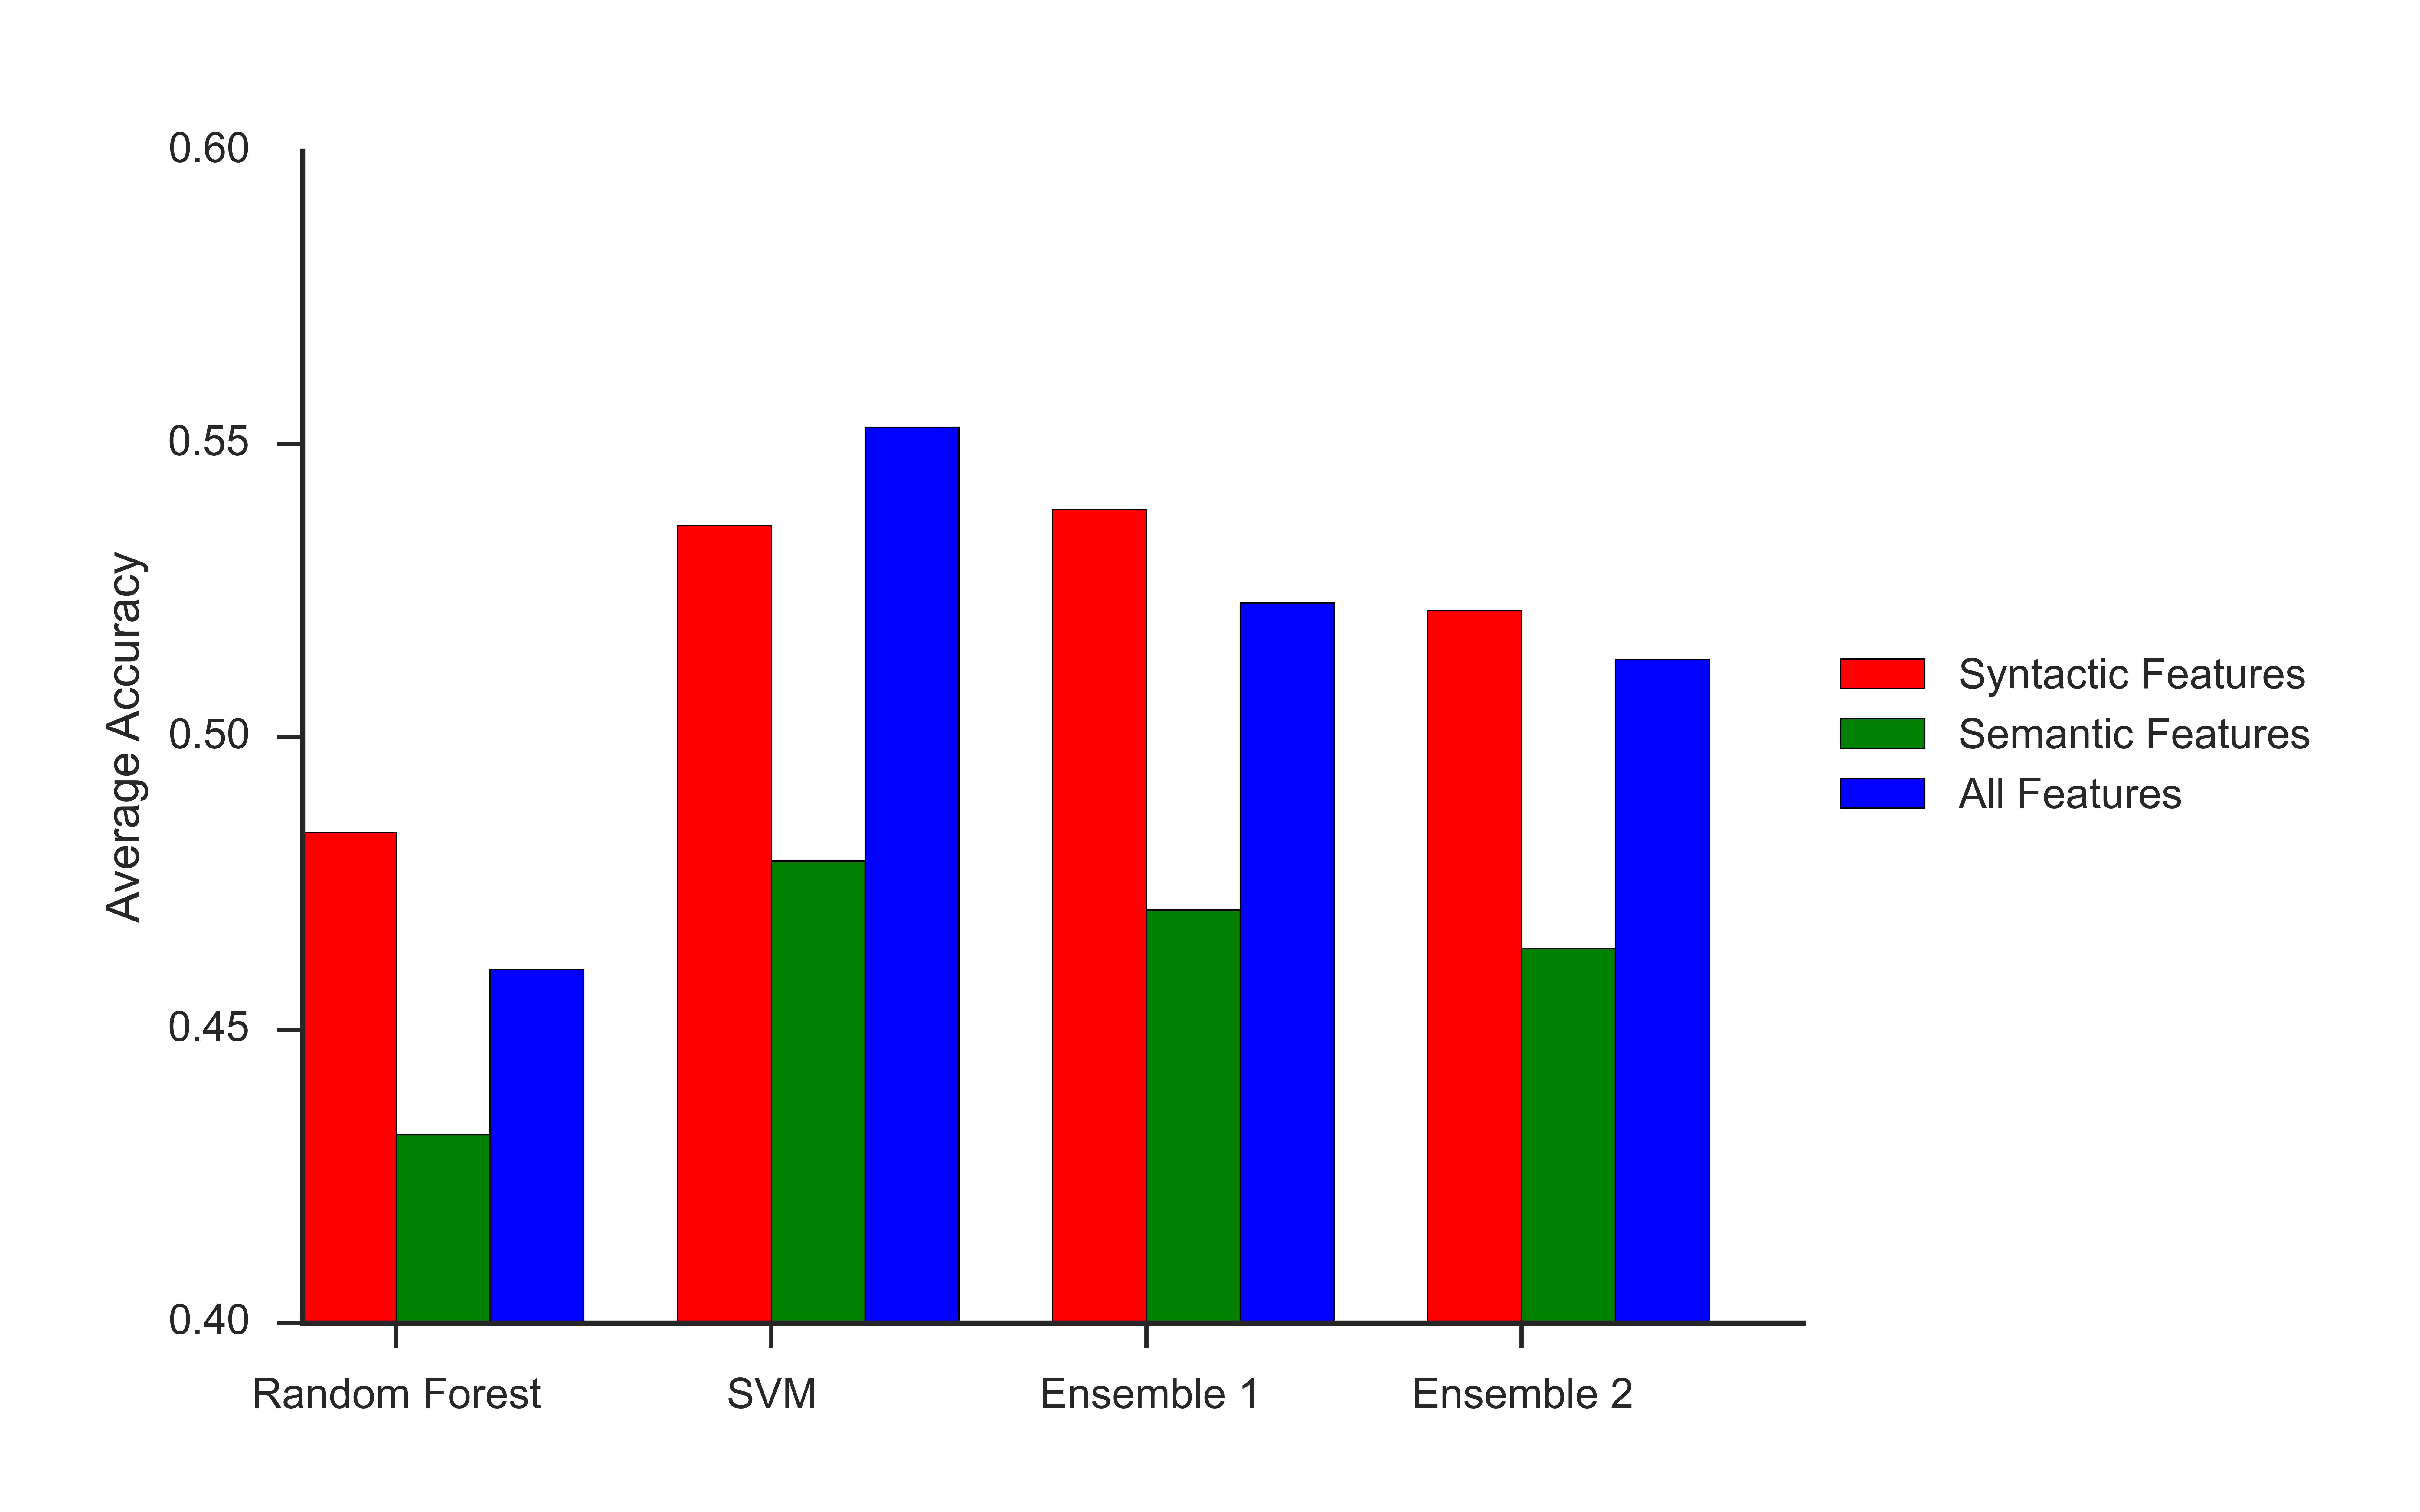
\includegraphics[width=.8\textwidth]{../graphics/plots/generous-a.png}
\end{figure}
\FloatBarrier

\begin{figure}[h!]
\caption{Accident-n}
\centering
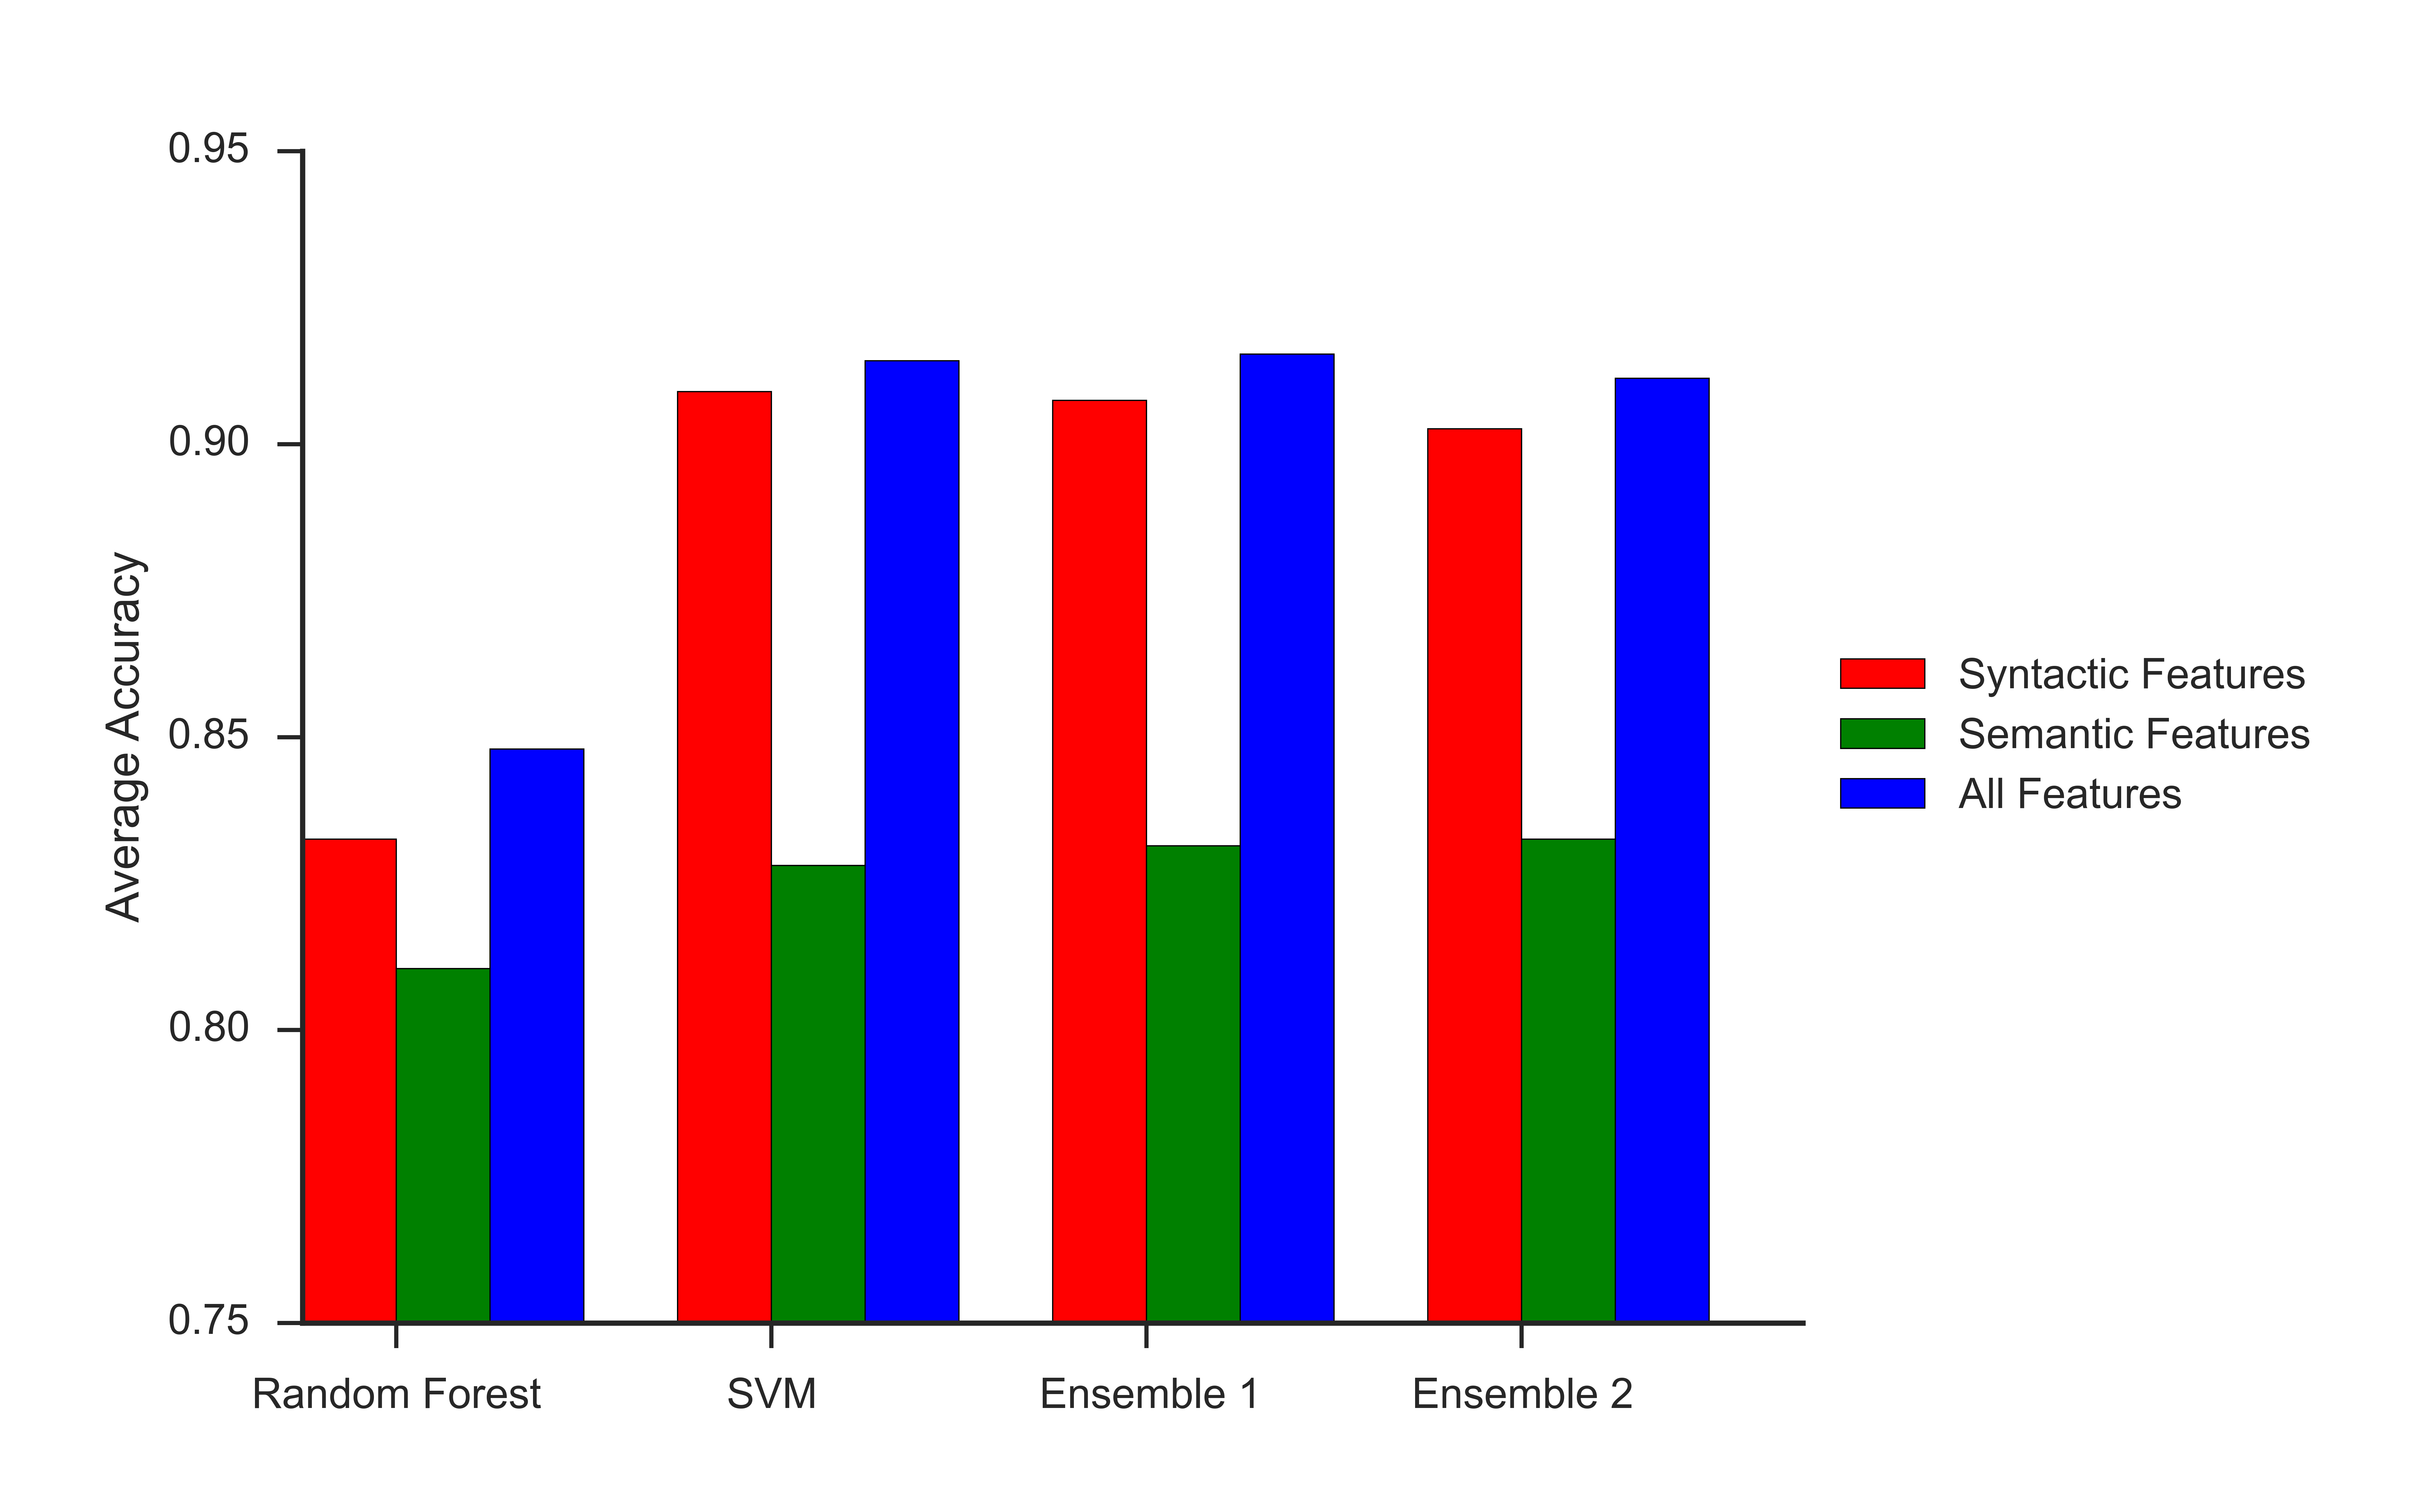
\includegraphics[width=.8\textwidth]{../graphics/plots/accident-n.png}
\end{figure}
\FloatBarrier

\begin{figure}[h!]
\caption{Float-v}
\centering
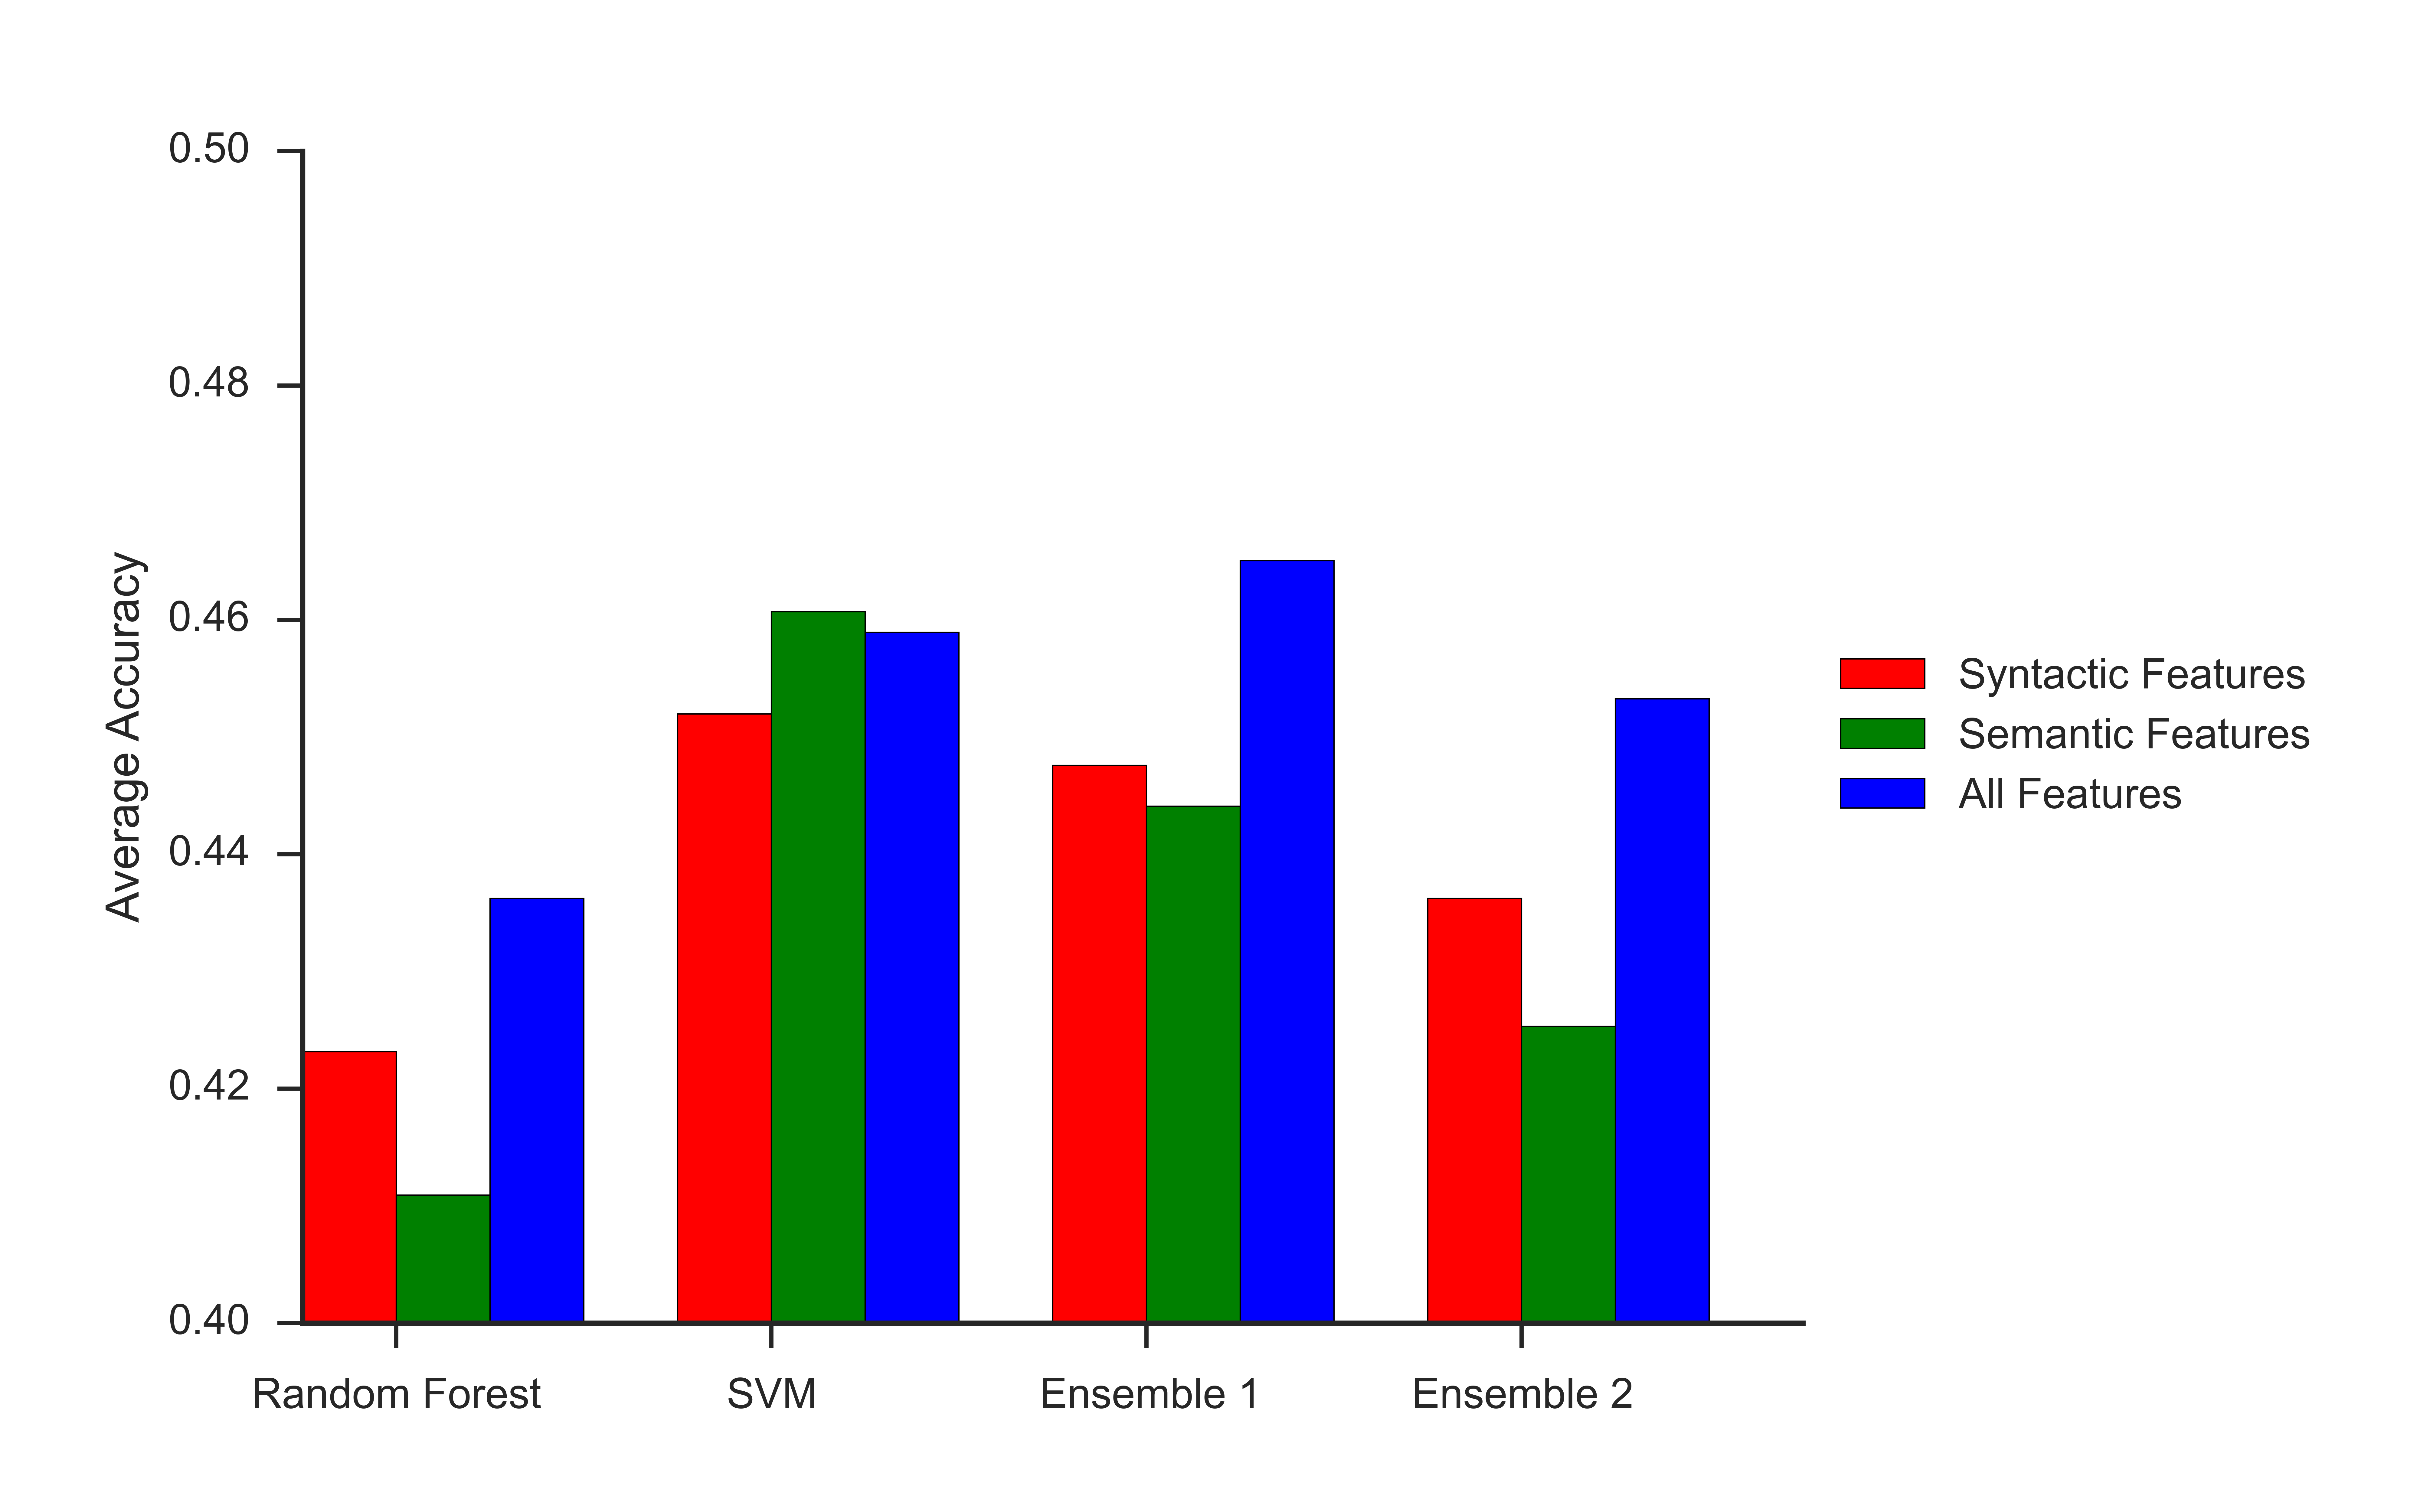
\includegraphics[width=.8\textwidth]{../graphics/plots/float-v.png}
\end{figure}
\FloatBarrier

\section{Discussion}

On average, our results do not suggest that including semantic features based on the AMR parse significantly improves WSD accuracy. For specific cases, though, we do show that semantic features improve accuracy in a statistically significant manner. In our discussion of semantic features we have shown why they make intuitive sense and should help increase WSD accuracy. Our average results may not have shown any change due to the fact that our AMR parser was trained on general web data as opposed to data more closely related to WSD.

We analyzed the importance of different semantic features based on the variable importance assigned to the features by the RF model. The top scoring features are as follows: triples of the form (node label, edge label, node label), label of the edges connected to the node representing the word of interest, label of nodes at a distance of three from the nodes of interest, label of the root node, and out degree of the node containing the word of interest. These features are not simply labels associated with some random node in the graph but they are strongly related to the nodes of interest (nodes representing the word to be disambiguated) or to the root node of the graph. This shows that semantic features contain cues to disambiguate word senses. Moreover, the performance of the models built using just the semantic features and the analysis of the top features indicate that there is information present in the AMR graph which can be exploited for this task.


\section{Related Work}

Pedersen and Mohammad\cite{pend} have shown that different learning algorithms are not very effective at increasing WSD accuracy on their own, and that the real boosts in accuracy come from feature engineering. In fact, they have shown how to achieve close to state-of-the-art results using the lexical and syntactic features we used in our model. We have extended this work by incorporating semantic features and have shown evidence that these additional features can increase performance for certain words. We have also provided evidence that the learning algorithm does matter with our results being stronger when using a SVM as opposed to a Random Forest.


\section{Future Work}

The major shortcoming of our work is that we don't show an improvement in accuracy across the board. We would like to investigate more deeply why certain words saw accuracy increases to determine if we can extract more efficient features from the AMR parse.
We think it would be good to explore training an AMR parser on data that is more closely related to the task of WSD. This should better help our semantic parse to represent the meaning with respect to ambiguous words. We would also like to use a  larger, more recent dataset to train and evaluate our system. 

Also, we believe that more time spent tuning the parameters of the learning algorithm could help us build better models. We could better optimize hyper-parameters as well as explore using a string kernel to see if it captures interesting patterns.


\section{Conclusion}

In this project, we explored the merits of using semantic features for the WSD task. We used a subset of Senseval 1 English Lexical Sample dataset for evaluation of our system. Our results suggest that the use of semantic features could prove beneficial for certain words and we hope that future research will make these results more generalizable. We believe that this is an avenue worth exploring as a topic of future research.

\newpage
\section{Appendix}

\begin{tabular}{lrrrrl}
\toprule
{} &  Random Forest &       SVM &  Ensemble 1 &  Ensemble 2 &         Word \\
\midrule
All Features       &       0.847940 &  0.914232 &    0.915356 &    0.911236 &   accident-n \\
Semantic Features  &       0.810487 &  0.828090 &    0.831461 &    0.832584 &   accident-n \\
Syntactic Features &       0.832584 &  0.908989 &    0.907491 &    0.902622 &   accident-n \\
All Features       &       0.675120 &  0.727273 &    0.749282 &    0.740191 &     bother-v \\
Semantic Features  &       0.547368 &  0.583254 &    0.581340 &    0.575598 &     bother-v \\
Syntactic Features &       0.685167 &  0.740670 &    0.765550 &    0.759330 &     bother-v \\
All Features       &       0.482969 &  0.499563 &    0.490393 &    0.488646 &  brilliant-a \\
Semantic Features  &       0.472052 &  0.504367 &    0.489956 &    0.489956 &  brilliant-a \\
Syntactic Features &       0.473799 &  0.503930 &    0.482096 &    0.482096 &  brilliant-a \\
All Features       &       0.635023 &  0.658986 &    0.671429 &    0.671889 &     derive-v \\
Semantic Features  &       0.596774 &  0.623963 &    0.621659 &    0.616590 &     derive-v \\
Syntactic Features &       0.646083 &  0.627650 &    0.670046 &    0.663594 &     derive-v \\
All Features       &       0.773656 &  0.856452 &    0.824194 &    0.806989 &     excess-n \\
Semantic Features  &       0.636559 &  0.673118 &    0.660753 &    0.650000 &     excess-n \\
Syntactic Features &       0.787097 &  0.851613 &    0.829570 &    0.819892 &     excess-n \\
All Features       &       0.436245 &  0.458952 &    0.465066 &    0.453275 &      float-v \\
Semantic Features  &       0.410917 &  0.460699 &    0.444105 &    0.425328 &      float-v \\
Syntactic Features &       0.423144 &  0.451965 &    0.447598 &    0.436245 &      float-v \\
All Features       &       0.460352 &  0.552863 &    0.522907 &    0.513216 &   generous-a \\
Semantic Features  &       0.432159 &  0.478855 &    0.470485 &    0.463877 &   generous-a \\
Syntactic Features &       0.483700 &  0.536123 &    0.538767 &    0.521586 &   generous-a \\
All Features       &       0.865625 &  0.884375 &    0.884821 &    0.884375 &    promise-v \\
Semantic Features  &       0.847321 &  0.854464 &    0.851339 &    0.850446 &    promise-v \\
Syntactic Features &       0.868304 &  0.871875 &    0.882589 &    0.882143 &    promise-v \\
All Features       &       0.770732 &  0.786585 &    0.802439 &    0.795122 &       sack-n \\
Semantic Features  &       0.651220 &  0.706098 &    0.692683 &    0.685366 &       sack-n \\
Syntactic Features &       0.787805 &  0.804878 &    0.809756 &    0.814634 &       sack-n \\
\bottomrule
\end{tabular} 

\begin{thebibliography}{9}

\bibitem{se}
http://www.senseval.org/

\bibitem{kh}
K.L. Lee and H.T. Ng.  2002.  An empirical evaluation of knowledge sources and learning algorithms for word sense disambiguation.   In Proceedings of the Conference on Empirical Methods in Natural Language Processing, pages 41-48.

\bibitem{pend}
Pedersen, Ted, Mohammad, Saif  "Combining Lexical and Syntactic Features for Supervised Word Sense Disambiguation." Proceedings of the Conference on Computational Natural Language Learning (CoNLL), May 6-7, 2004, Boston, MA.

\bibitem{amr}
"Abstract Meaning Representation for Sembanking" (L. Banarescu, C. Bonial, S. Cai, M. Georgescu, K. Griffitt, U. Hermjakob, K. Knight, P. Koehn, M. Palmer, N. Schneider), Proc. Linguistic Annotation Workshop, 2013. 

\bibitem{jamr}
JAMR - AMR Parser: https://github.com/jflanigan/jamr.

\bibitem{syntalex}
Proceedings of the Third International Workshop on the Evaluation of Systems for the Semantic Analysis of Text (Senseval-3), pp. 159-162, July 25-26, 2004, Barcelona, Spain. 

\bibitem{sp}
Dan Klein and Christopher D. Manning. 2003. Accurate Unlexicalized Parsing. Proceedings of the 41st Meeting of the Association for Computational Linguistics, pp. 423-430. 

\bibitem{data}
http://www.d.umn.edu/~tpederse/data.html.

\bibitem{recall}
Edmonds, Philip. "SENSEVAL: The evaluation of word sense disambiguation systems." ELRA newsletter 7.3 (2002): 5-14.

\bibitem{prop}
P. Kingsbury and M. Palmer. 2002. From TreeBank to PropBank. In Proc. LREC.

\end{thebibliography}

\end{document}






\begin{table}[h]
\begin{tabular}{l|lll}
\hline
Word      & Part of Speech & Training Size & Testing Size \\ \hline
Excess    & N              & 178           & 186          \\
Float     & V              & 183           & 229          \\
Brilliant & A              & 441           & 229          \\ 
Accident  & N              & 1,234         & 267          \\
Promise   & V              & 1,163         &   224          
\end{tabular}
\end{table}

\begin{table}[h]
\begin{tabular}{l|l}
\hline
Word      & Senseval Average  \\ \hline
Excess    & 0.652                     \\
Float     & 0.402                      \\
Brilliant & 0.443                      \\ 
Accident  & 0.802                   \\
Promise   & 0.741                      
\end{tabular}
\end{table}

\begin{verbatim}
(d / describe-01
    :arg0 (m / man)
    :arg1 (m2 / mission)
    :arg2 (d / disaster))
\end{verbatim}

\vspace{4mm}
The accident appeared to have little effect on the Christmas party, except to lengthen it considerably.
\vspace{4mm}

\noindent


  